\documentclass[a0,portrait]{a0poster}
%\usepackage[spanish]{babel}
\usepackage[utf8]{inputenc}


\usepackage{times,colordvi,amsmath,epsfig,float,color,multicol}

\pagestyle{empty}
\setlength{\parindent}{0cm}
\setlength{\parskip}{2ex}
\setlength{\columnsep}{3cm}
\addtolength{\textwidth}{2cm}
\addtolength{\oddsidemargin}{-1.5cm}

\renewcommand{\normalsize}{\Large}
\def\regularsize{\@setfontsize\normalsize{34pt}{37}}

\renewcommand\refname{}
\setlength{\fboxrule}{0.1cm}


% ----------------------------------------------------------------


% PMS287 CMYK=[100% 69% 0% 11.5%] RGB=[38/256 67/256 151/256]
\definecolor{qmuldarkblue}{rgb}{0.1484375,0.26171875,0.58984375}

\definecolor{backgrey}{rgb}{0.93,0.93,0.93}
\definecolor{backblue}{rgb}{0.93,0.93,1}
\definecolor{backyellow}{rgb}{1,1,0.88}

\definecolor{backred}{rgb}{1,0.9,0.9}
\definecolor{backgreen}{rgb}{0.9,1,0.9}
\definecolor{backpink}{rgb}{1,0.9,1}
\definecolor{backturquoise}{rgb}{0.9,1,1}


% ----------------------------------------------------------------


\makeatletter
\renewcommand{\section}{\@startsection
        {section}                          % the name
        {1}                                % the level
        {0mm}                              % the indent
        {-0.7\baselineskip}                % the beforeskip
        {5mm}                              % the afterskip
        {\center\huge\color{qmuldarkblue}\bfseries}} % the style
\renewcommand{\subsection}{\@startsection
        {subsection}                          % the name
        {2}                                % the level
        {0mm}                              % the indent
        {-0.7\baselineskip}                % the beforeskip
        {5mm}                              % the afterskip
        {\center\Large\color{qmuldarkblue}\bfseries}} % the style

\makeatother


\usepackage{theorem}
{\theorembodyfont{\rmfamily}%
%\newtheorem{ejemplo}{Ejemplo}[section]}
%\usepackage{Sweave}

\begin{document}

%\vspace{1cm}

\colorbox{qmuldarkblue}{
 \color{white}
 
\begin{minipage}{0.2\textwidth}
\begin{center}
 \vskip 1cm
	
  
\includegraphics[width=8cm]{images/IBSVictoria.png}
% Session Number \\ (\textit{t.b.a. by the organizers})   

%     \textit{	XXVIII International Biometric Conference}	Victoria, Canadà
     \end{center}
     
\end{minipage}


\begin{minipage}{0.6\textwidth}
\vspace*{0.4cm}
\begin{center}
   \textrm
   {
    {\huge \bf \em Integrative Analysis to Select Genes Regulated by Methylation in a Cancer Colon Study}\\[1ex]
    {\large Sánchez-Pla, Alex$^{1,3}$, Ruiz de Villa, M. Carme$^1$, Carmona, Francesc$^1$, Bazzoco, Sara$^2$,  
Arango, Diego$^2$}\\[1ex]
    {\large $^1$ Departament of Genetics Microbiology and Statistics, Universitad de Barcelona\\
    $^2$ CIBBIM-Nanomedicine. Biomedical Research in Digestive Tumors, (VHIR), Barcelona\\
    $^3$ Statistic and Bioinformatics Unit. Vall d'Hebron Research Institute.  (VHIR). Barcelona}
   }
   \end{center}
   
\vspace*{0.4cm}
\end{minipage}

\begin{minipage}{0.2\textwidth}
\begin{center}
   
\includegraphics[width=14cm]{images/allLogos.png}
   \end{center}
\end{minipage}
}
%\vspace{0.5cm}


% ----------------------------------------------------------------


\begin{multicols}{2}

\fcolorbox{black}{white}{\parbox{1.0\columnwidth}
{
\section{Introduction}

\begin{itemize}
\item Methylation %of CpG dinucleotides in the promoter 
of genes involved in the oncogenic process is a key process contributing to tumor initiation and/or progression\cite{sadikovic:2008}. 

\item Finding \textit{Genes Regulated by Methylation} or GRM can lead to a better understanding and be a guide to finding new drug targets.

\item This study originates in a work searching for colon cancer biomarkers \cite{bazzocco}. Cell lines with increasing sensitivity to a chemotherapy drug, were analyzed with Expression and Methylation arrays.  Finding GRM was used to search of candidate genes for new therapies.

\item In cancer--related genes it is common to observe a decrease in gene expression associated with hypermethylation. Methylation is often described as a binary on-off signal (\cite{Liu})
that is, when methylation is ``off'' the gene can express normally and
its expression will be low or high, whereas when methylation
is ``on'', the expression of the gene will be \emph{repressed} and its
values will tend to be low.

\item As a consequence of this \emph{high-methylation/low-expression} and
\emph{low-methylation/high-expression} relation plots depicting 
methylation and expression will show L--shape patterns so the
strategy adopted will be to mine such plots and select those that
have such a shape.

\end{itemize}

}}

\begin{center}
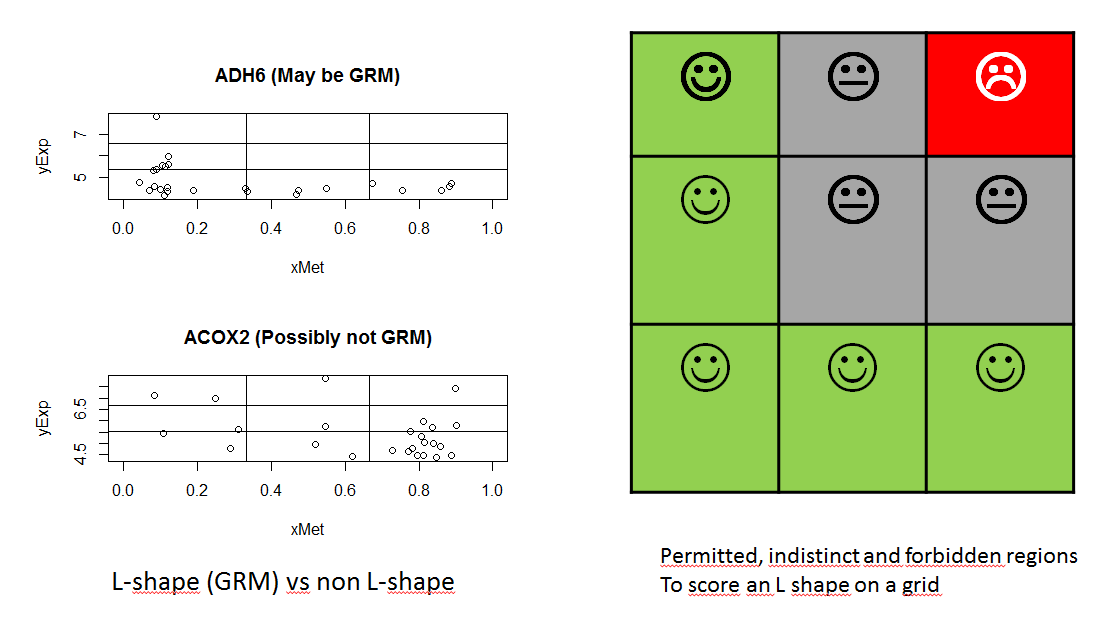
\includegraphics[width=0.9\columnwidth]{./images/Lshapes_1and2.png}
\end{center}

\fcolorbox{black}{backblue}{\parbox{1.0\columnwidth}
{\section{Objectives}

\begin{itemize}
\item Study how gene expression is regulated by methylation in a set of colon cancer cell lines.
\item Set up a method to detect the level of methylation at which a gene can be considered regulated by methylation (to be ``on").
\item Compare this method with other that have been developed to
  \begin{itemize}
  \item detect methylation thresholds and
  \item detect patterns in scatterplots.
  \end{itemize} 
\end{itemize} 
}}

\vspace{0.1cm} 
\fcolorbox{black}{backgrey}{\parbox{1.0\columnwidth}
{\section{Methods}
\subsection{Using Conditional Mutual Information}
\begin{itemize}
\item Following \cite{Liu} in order to determine whether methylation $X$ and expression $Y$ of a gene exhibit an L--shape, the conditional Mutual Information $cMI(t)$ for different choices of threshold $t$ is computed.
\[
\mathit{cMI}(t)=I(X,Y|X>t)P(X>t) + I(X,Y|X\le t)P(X\le t)
\]
\item If the relation between methylation and expression shows an L-shape  as $t$ moves from 0 to 1, $\mathit{cMI}(t)$ first decreases and then increases, its value approaching zero when $t$ coincides with the reflection point. 
\end{itemize}
}}

%\vspace{0.6cm} 
\fcolorbox{black}{backgrey}{\parbox{1.0\columnwidth}
{\begin{itemize}
\item For an L-shape gene it is verified that:
\begin{itemize}
\item The ratio $r=\frac{\min\{\mathit{cMI}(t)\}}{\mathit{cMI}(0)}$ is small, 
\item $t^{\ast} = \mathrm{argmin}\{ \mathit{cMI}(t) \}$ is the \textbf{optimal threshold} for 
dichotomizing the methylation data of this gene.
\end{itemize}
\end{itemize}

%To estimate the MI terms we use a kernel-based estimator by applying a %Gaussian kernel to each data point:
%\[
%I(X,Y) = \frac 1M \sum_{i=1}^M \log\frac{M\sum_{j=1}^M e^{-\frac{1}{2h^2}%((x_i-x_j)^2+(y_i-y_j)^2)}}{%
      %                                \sum_{j=1}^M e^{-\frac{1}{2h^2}(x_i-%x_j)^2} \sum_{j=1}^M e^{-\frac{1}{2h^2}(y_i-y_j)^2}}
%\]
%where $h$ is a tuning parameter for the kernel width empirically set to 
% $h=0.3$.
  

\subsection{Based on Spline regression}
\begin{itemize}
\item As an alternative to the previous method we suggest that spline regression \cite{racine} can be used for scatter plot clustering.
\item In spline regression a curve $y=s(x)$ is represented as $\mathbf{y}_i=\mathbf{B}_i\mathbf{c}$ where 
\begin{itemize}
\item $\mathbf{B}_i =\left[ B_{1p}\mathbf{x}_i,B_{2p}\mathbf{x}_i,\dots,B_{Lp}\mathbf{x}_i \right]$ the spline basis matrix and 
\item $\mathbf{c}$ is the vector of spline coefficients.
\end{itemize}

\item This suggests the following method (and algorithm) for detecting L--shaped genes based on \textbf{Clustering Spline Coefficients}:
\begin {enumerate}
\item Select genes with significant correlation.
\item For each selected gene fit a cubic splines regression model.
\item Obtain a distance matrix between all genes using the $1-\rho$ distance computed on spline coefficients.
\item Perform a hierarchical clustering and 
\item Select genes in the \textit{L-shaped cluster(s)}.
\end{enumerate}
\end{itemize}
}}

\fcolorbox{black}{backgrey}{\parbox{1.0\columnwidth}
	{\subsection{Heuristic approach}
A heuristic method has been developed basing on imitating the visual selection of L-shapes (see figure)
\begin{itemize}
\item Overimpose a $3\times 3$ grid on the scatterplot.
\item Score points on each subgrid in such a way that
\begin{itemize}
	\item Points in permitted regions increase score
	\item Points in non-desired regions decrease score
	\item Points in non-allowed regions set score to $\-infty$.
\end{itemize}
\item Use cross-validation to tune scoring parameters.
\end{itemize}

\subsection{The Naive method}

Traditionally selection has been based on searching for genes with negative correlation betweem expression and correlation. This ``Naïve approach" is used to compare with other approaches.
}}

% \vspace{0.6cm}
\fcolorbox{black}{backyellow}{\parbox{1.0\columnwidth}
{\section{Results}

\begin {itemize}
% After the previous selection of genes we worked with 191 genes
% decided to choose 5 clusters
\item Spline regression:
 The 2 first clusters included the genes with an L-shape

\begin{center}
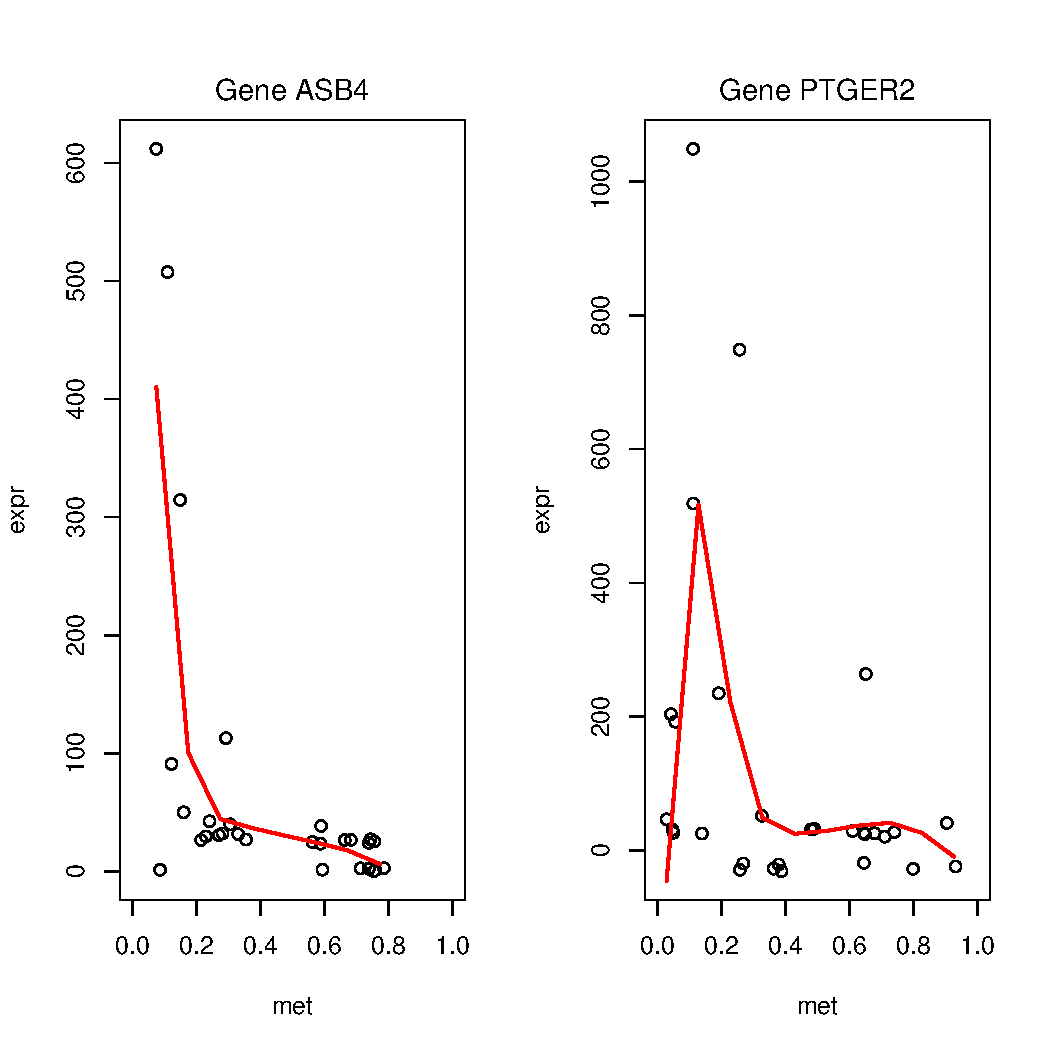
\includegraphics[width=0.3\columnwidth]{./images/grafic_two_patterns.pdf}
\end{center}

\item Conditional Mutual Information

% No previous selection of the genes was needed
%\begin{block}{Three criteria}
We filtered for L-shapes using a combination of three criteria:
\begin{itemize}
\item the ratio $r<0.25$
\item unconditioned MI $\mathit{cMI}(0)>0.1$
\item the median expression on the left side of the optimal threshold $t^{\ast}$ is higher
than the median expression on the right side.
\end{itemize}
%\end{block}
% The parameters are chosen according to a random permutation test (see Liu(2012)).
% According to the above criteria, a total of 641 genes are selected to be L-shape genes.


\item Comparison between the methods:
\begin{center}
\begin{tabular}{|c|c|c|}
\hline
Initial selection & 191 & 641 \\
\hline
\hline
Cluster & Splines & cMI \\
\hline
1 & 140 & 102 \\
2 & 22 & 16 \\
\hline
Total & 162 & 118 \\
\hline 
\end{tabular}
\end{center}

\item In summary...
  \begin{itemize}
  \item We have found similar results between both methods.
  \item Biological interpretation is in progress but preliminary (unpublished) results are consistent with the hypothesis.
  \item Sample size is a limiting factor: $cMI$ works better with hundreds of samples but one may have a very small number (real cases: 30, 12)
\end{itemize}

%\begin{center}
%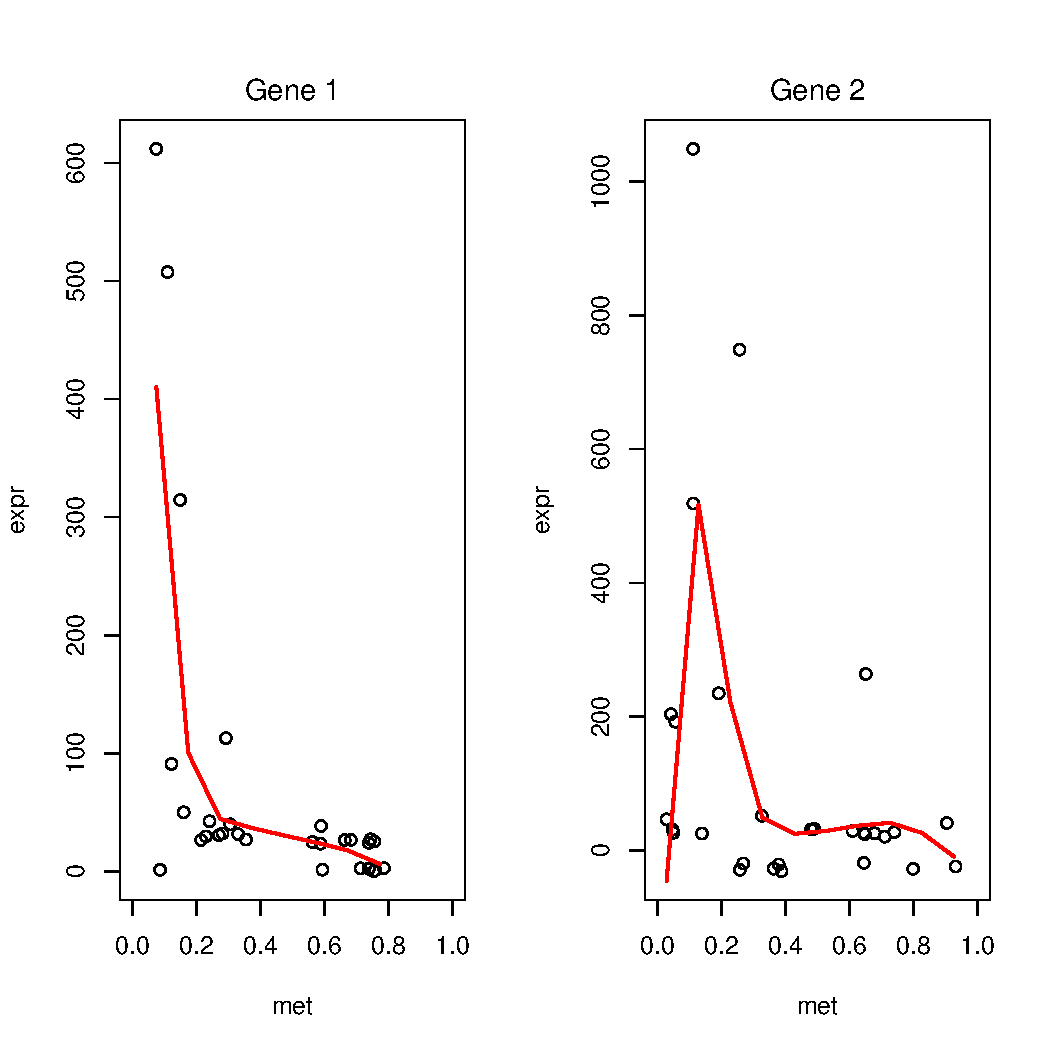
\includegraphics[width=0.6\columnwidth]{./images/grafic_two_genes.pdf}
%\end{center}

\end{itemize}


}}

%\vspace{1cm} \fcolorbox{black}{white}{\parbox{1.0\columnwidth}
%{\input{sectionsUseR/conc}}}

%\vspace{0.2cm} 
\small\vspace{-5mm}
\begin{thebibliography}{9}
%\addcontentsline{toc}{chapter}{\numberline{}Bibliografía}
%
%\bibitem{cohen} J. Cohen, \emph{Statistical power analysis for the behavioral sciences} (2nd ed.). % Hillsdale,NJ: Lawrence Erlbaum, 1988.

%\bibitem{faraway} J.J. Faraway, \emph{Linear Models with R}, Chapman \& Hall/CRC, 2004.

%\bibitem{montgomery} D.C Montgomery \emph{Design and Analysis of Experiments}, John Wiley \& Sons, 2008.

%\bibitem{blog} \texttt{http://erre-que-erre-paco.blogspot.com.es/2013/04/el-codigo-body-td-font-family-sans.html}

\bibitem{bazzocco} Sarah Bazzocco, Hafid Alazzouzi, M. Carme Ruiz de Villa, Alex Sanchez-Pla, John M. Mariadason, Diego Arango (2013) \emph{Genome-Wide Analysis of DNA Methylation in Colorectal Cancer}. Submitted.

\bibitem{Liu} Yihua Liu and Peng Qiu. (2012) \emph{Integrative analysis of methylation and gene expression data in TCGA} IEEE International Workshop on Genomic Signal Processing and Statistics (GENSIPS)

\bibitem{racine} Jeffrey Racine. (2012) A primer on regression splines.\newline
\verb|http://cran.r-project.org/web/packages/crs/vignettes/spline_primer.pdf|

\bibitem{sadikovic:2008}
B~Sadikovic, K~Al-Romaih, J.A Squire, and M~Zielenska.
\newblock {Cause and {Consequences} of {Genetic} and {Epigenetic} {Alterations}
	in {Human} {Cancer}}.
\newblock {\em Current Genomics}, 9(6):394--408, September 2008.

\end{thebibliography}
\normalsize

\end{multicols}


% ----------------------------------------------------------------

%\vspace{0.5cm}

\colorbox{qmuldarkblue}
{
 \color{white}
 \parbox{1.0\textwidth}
 {
 % \vspace{0.2cm}

  \begin{center}
21st Annual International Conference on Intelligent Systems for Molecular Biology \hspace{2cm}
12th European Conference on Computational Biology
  \end{center}
%  \vspace{0.2cm}
 }
}


\end{document}
